\documentclass[12pt,a4paper,fleqn]{article}

\usepackage[utf8]{inputenc}
\usepackage[french]{babel}
\usepackage{tikz}
\usetikzlibrary{positioning}
\usetikzlibrary{decorations.markings}
\usepackage[T1]{fontenc}
\usepackage{amsmath}																				% les maths
\usepackage{amsfonts}
\usepackage{amssymb}
\usepackage{fourier}																					% symboles intégral propre
\usepackage{graphicx}
\usepackage[left=2cm,right=2cm,top=2cm,bottom=2cm]{geometry}	% les marges
\usepackage{multicol}																					% pour écrire sur plusieurs colones
\usepackage{setspace}																				% set space between lines
\usepackage{array}																						% stretch array lines
\usepackage[hyphens]{url}
%\usepackage[hyphenbreaks]{breakurl}														% for long urls
\usepackage{chemfig}																					% pour les formules chimiques


\usepackage[breaklinks]{hyperref}															% clickable links
\hypersetup{
    colorlinks=true,
    linkcolor=red_f,
    citecolor=bleu_f,
    filecolor=green_f,
    urlcolor=bleu_f
}

\usepackage{xcolor}																			% colors
\usepackage[framemethod=tikz]{mdframed}									% fancy environments

\usepackage{siunitx}																					% écriture des nombres et unités
\sisetup{
locale = FR,
input-product=*, % enable to type equation as in Python
per-mode = symbol,%reciprocal,
exponent-product = \times, % replace by \cdot if desired
quotient-mode = fraction,
scientific-notation=false, % if desired
separate-uncertainty = true,
output-complex-root = j, % or i
number-unit-product = \, ,
load-configurations = abbreviations
}

%%%%%%%%%% graphic charter

\renewcommand{\familydefault}{\sfdefault}												% sans serif font

%%%%% HEADER
%\pagestyle{fancy}
%\lhead{\textcolor{gray_f}{Physique-Chimie\\R. METZDORFF}}
%\chead{\textcolor{gray_f}{Lycée Suzanne Valadon}}
%\rhead{\textcolor{gray_f}{2020-2021}}
%\renewcommand{\headrulewidth}{0.4pt}
%\let\HeadRule\headrule
%\renewcommand\headrule{\color{gray_f}\HeadRule}

%%%%% COLORS
\definecolor{gray_f}{RGB}{68,84,106}
\definecolor{gray_c}{RGB}{214,220,229}
\definecolor{gray_cc}{RGB}{245,245,245}
\definecolor{bleu_f}{RGB}{91,155,213}
\definecolor{bleu_c}{RGB}{222,235,247}
\definecolor{red_f}{RGB}{204,0,0}
\definecolor{red_c}{RGB}{245,204,204}
\definecolor{orange_f}{RGB}{237,125,49}
\definecolor{orange_c}{RGB}{251,229,214}
\definecolor{green_f}{RGB}{112,173,71}
\definecolor{green_c}{RGB}{226,240,217}
\definecolor{yellow_f}{RGB}{255,192,0}
\definecolor{yellow_c}{RGB}{255,242,204}
\definecolor{code_keyword}{RGB}{23,23,139}										% colors for pyhton code
\definecolor{code_comment}{RGB}{50,137,21}
\definecolor{code_string}{RGB}{139,139,25}
\definecolor{red_unilim}{RGB}{166,41,41}
\definecolor{gray_unilim}{RGB}{78,87,94}
\definecolor{orange_unilim}{RGB}{209,98,40}

%%%%% NEW ENVIRONMENTS

%%% header
\mdfdefinestyle{s_head}{%
	linecolor=red_unilim!,
	outerlinewidth=3pt,%
	frametitlerule=false,
	topline=false,
	bottomline=false,
	rightline=false,
	leftline=false,
	backgroundcolor=red_unilim,
	innertopmargin=8pt,
	roundcorner=0pt,
	nobreak=true,
	fontcolor=white
}
\newmdenv[style=s_head]{header_env}
\newenvironment{header}
{%\stepcounter{exa}%
	\addcontentsline{ldf}{figure}{0}%
	\begin{header_env}\qquad\Large\bf}
	{\end{header_env}}

%%%%% New command

\newcommand{\app}{\colorbox{bleu_c}{\textcolor{bleu_f}{APP}}}
\newcommand{\rea}{\colorbox{yellow_c}{\textcolor{yellow_f}{REA}}}
\newcommand{\anarai}{\colorbox{green_c}{\textcolor{green_f}{ANA-RAI}}}
\newcommand{\val}{\colorbox{orange_c}{\textcolor{orange_f}{VAL}}}
\newcommand{\com}{\colorbox{red_c}{\textcolor{red_f}{COM}}}
\newcommand{\auto}{\colorbox{white}{\textcolor{black}{AUTO}}}
\newcommand{\rco}{\colorbox{gray_c}{\textcolor{gray_f}{RCO}}}


\bibliographystyle{custom-bib/thesis}
\usepackage{bibentry}
\usepackage{pdfpages}

\newcommand{\ex}{\vec{e}_x}
\newcommand{\ey}{\vec{e}_y}
\newcommand{\ez}{\vec{e}_z}

\renewcommand{\d}{\mathrm{d}}
\newcommand{\cad}{c'est-à-dire}

\begin{document}

\begin{header}
\begin{minipage}{0.55\textwidth}
Rapport de Master 2
\end{minipage}
\begin{minipage}{0.38\textwidth}
\href{https://www.unilim.fr/}{
\includegraphics[scale=1]{logo.png}}
\end{minipage}
\end{header}

\vspace{30pt}
\begin{spacing}{1.2}
{\bf
\begin{Large}
\noindent
\textcolor{gray_unilim}{INSPE Académie de Limoges}
\end{Large}

\begin{large}
\noindent
\textcolor{gray_unilim}{Métiers de l'enseignement, de l'éducation et de la formation}

\noindent
\textcolor{gray_unilim}{Master MEEF Second degré}

\noindent
\textcolor{gray_unilim}{Professeur de Physique et de Chimie}

\noindent
\textcolor{gray_unilim}{Didactique, épistémologie et histoire des sciences}

\end{large}
}

\vspace{20pt}

\noindent
\textcolor{gray_unilim}{2020--2021}

\vspace{40pt}
\begin{large}
\bf
\noindent
\textcolor{gray_unilim}{Galvanomètres}

\vspace{150pt}
\noindent
\textcolor{gray_unilim}{Antoine \textsc{Eggenspiller}}

\noindent
\textcolor{gray_unilim}{Collège Guy de Maupassant}

\vspace{\baselineskip}

\noindent
\textcolor{gray_unilim}{Rémi Metzdorff}

\noindent
\textcolor{gray_unilim}{Lycée Suzanne Valadon}
\end{large}
\end{spacing}

\vfill

\hfill

\includegraphics[scale=1]{logo_bottom.png}

\thispagestyle{empty}
\newpage

\tableofcontents
\newpage



\section*{Introduction}
\addcontentsline{toc}{section}{Introduction}

Ce rapport présente le fonctionnement et la restauration de deux galvanomètres datant du début du XX\textsuperscript{ème} siècle.
Il s'agit d'un ampèremètre et d'un voltmètre produits par Chauvin et Arnoux.
Les détails concernant l'historique de ces appareils sont présentés extensivement dans un précédent rapport \cite{Ardellier2016} et ne seront pas repris ici.
La première section s'intéresse au principe de fonctionnement du galvanomètre et en présente un modèle simplifié.
La restauration des deux appareils est ensuite détaillée.
Finalement, une expérience simple impliquant les deux instruments est présentée.


\section{Principe de fonctionnement}

\subsection{Principe général}

\begin{figure}[htbp]
    \center
    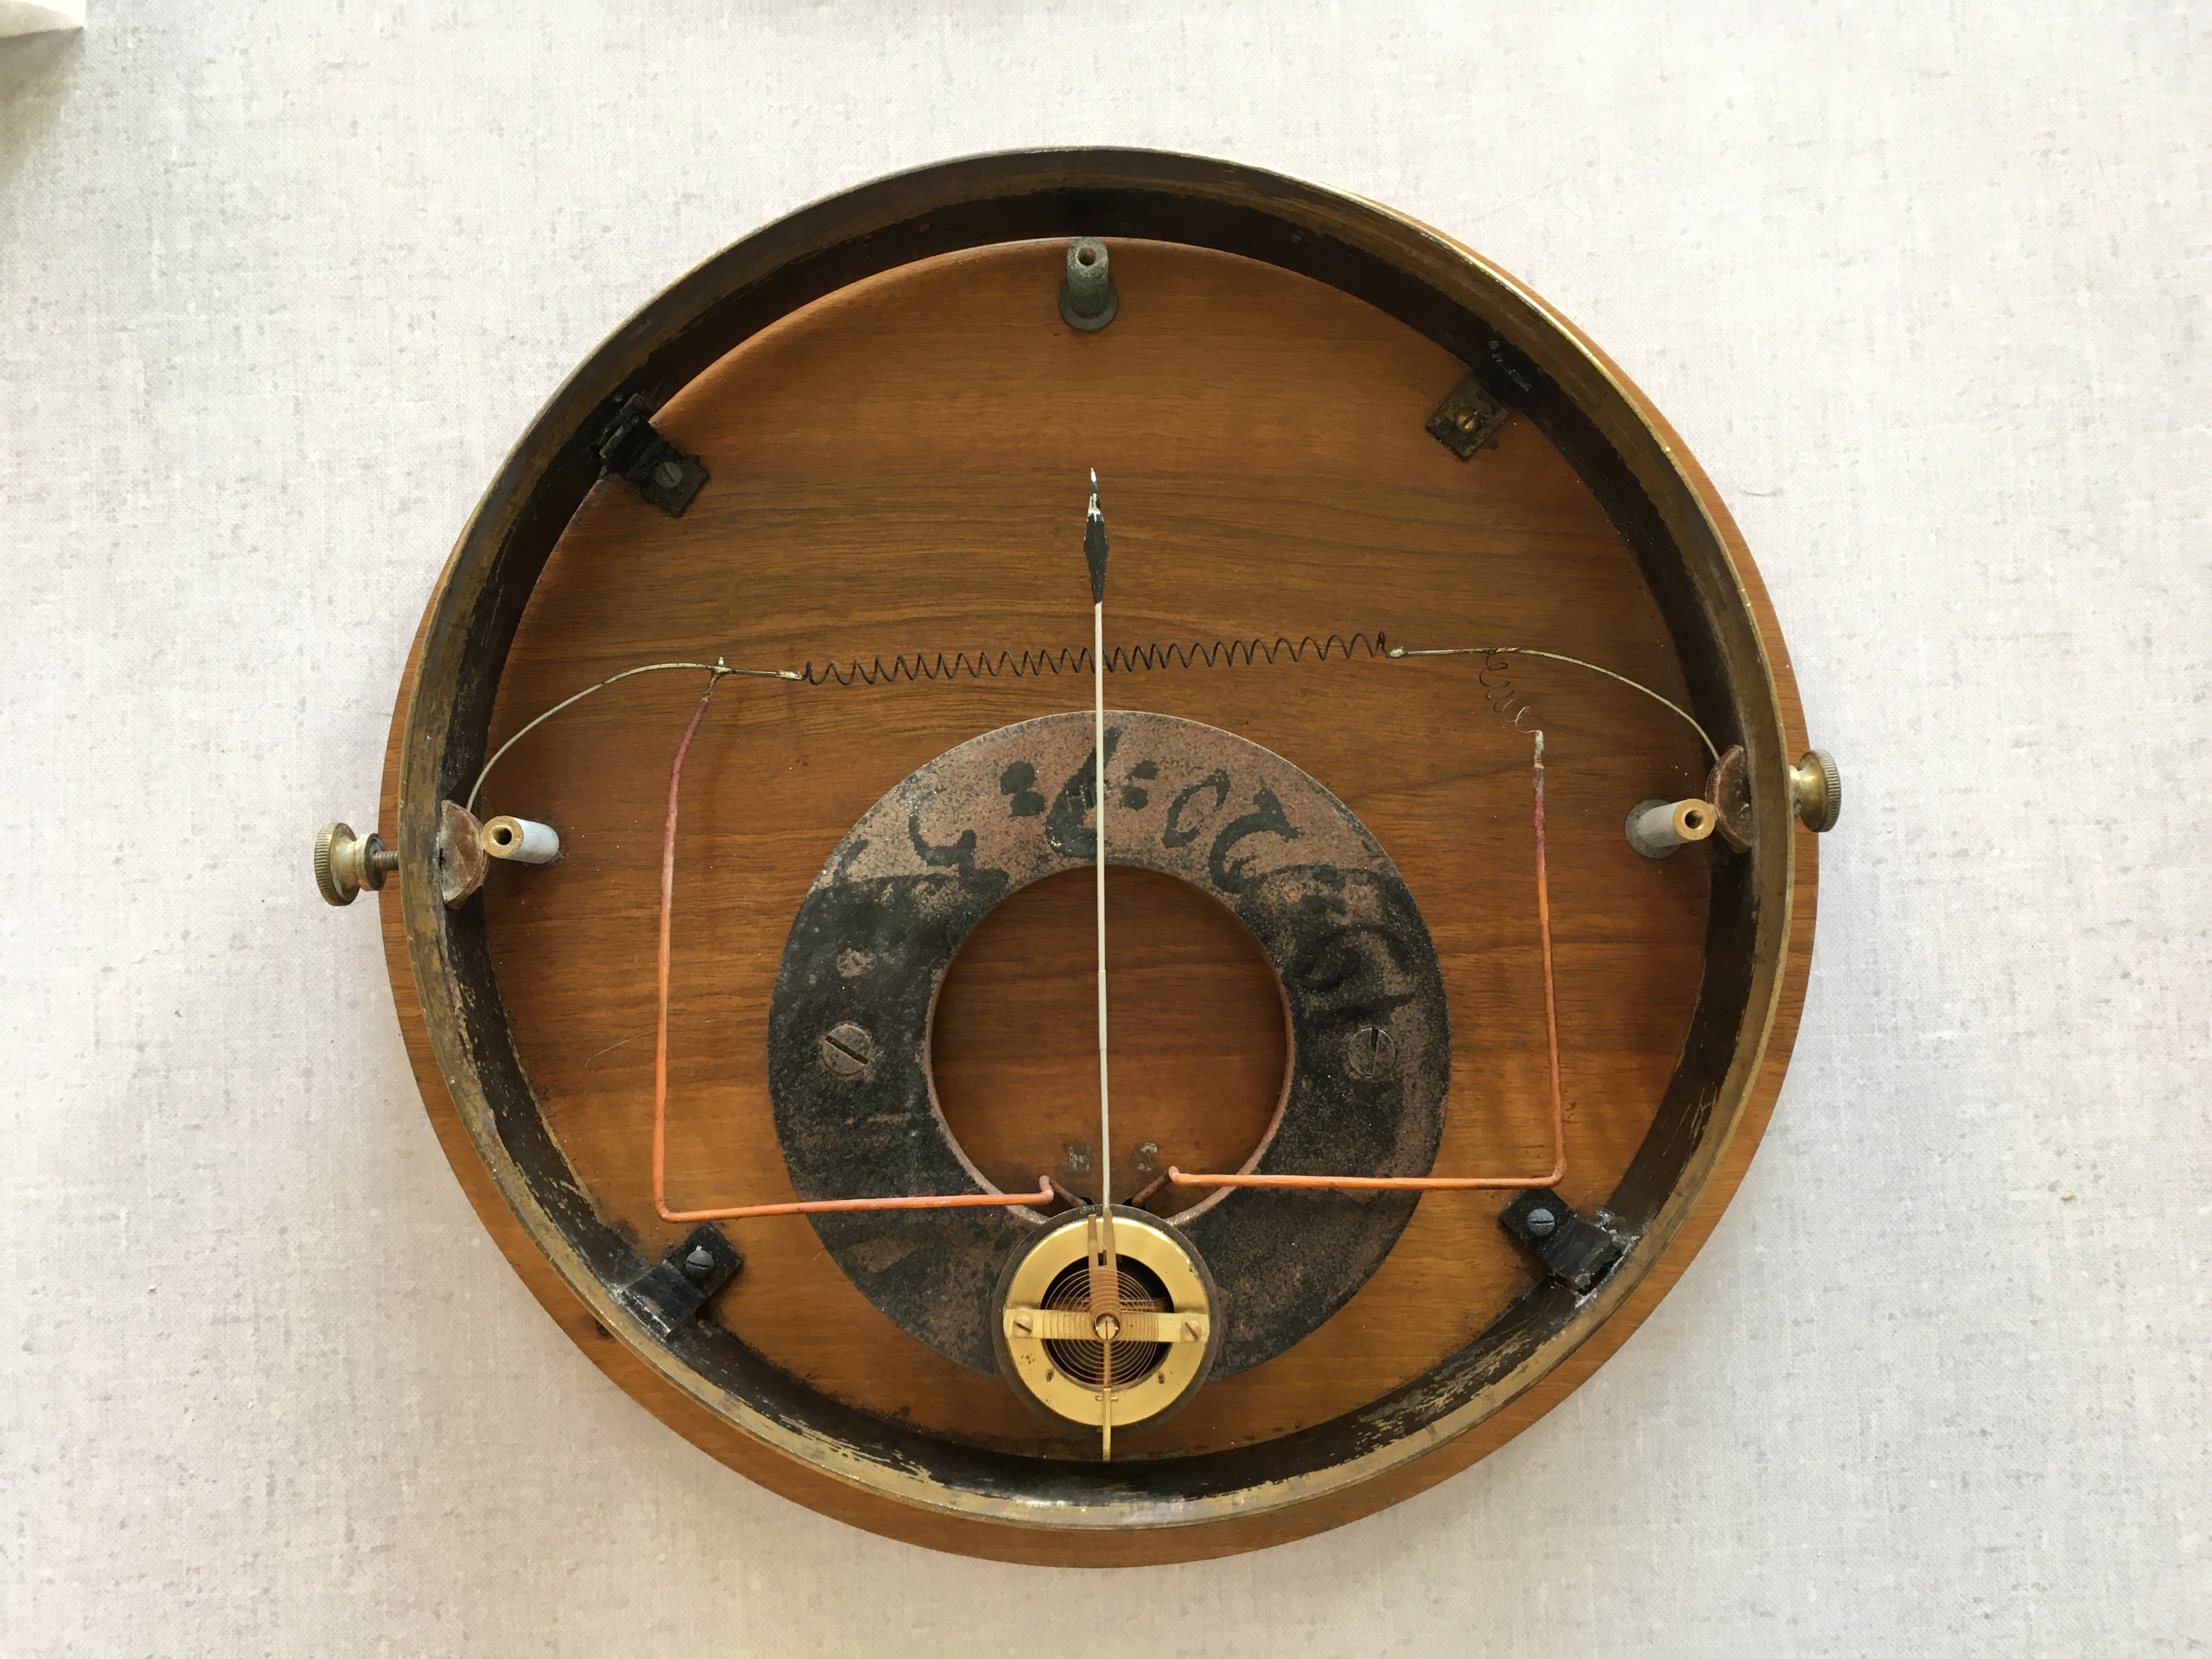
\includegraphics[trim=1300 300 1300 800, clip, width=.5\linewidth]{images/IMG_4037.JPG}
    \caption{
    Le \og cœur \fg{} du galvanomètre.
    Le champ magnétique est produit par l'aimant permanent torique.
    La cadre mobile, situé dans l'entrefer de l'aimant, est caché derrière un ressort en spirale qui maintient l'aiguille au centre du cadrant en l'absence de courant électrique.
    Les deux fils situés de part et d'autre du cadre alimentent la bobine.
    Le fil fin en forme de ressort est propre à l'ampèremètre : il n'est pas indispensable au fonctionnement du galvanomètre et son rôle sera expliqué plus tard.}
    \label{fig:principe}
\end{figure}

Il existe plusieurs types de galvanomètres adaptés à différents usages.
Ceux présentés ici sont dit à \emph{cadre mobile}.
\og \emph{Ces galvanomètres sont basés sur le principe d'un cadre galvanométrique mobile dans un champ magnétique produit par un aimant permanent} \fg{}, comme l'explique la notice du fabriquant (Ann.~\ref{ann:catalogue}).
Le cadre galvanométrique est un circuit qui prend la forme d'une bobine de fil de cuivre : lorsqu'elle est parcourue par un courant $I$, l'action du champ magnétique se traduit par une force de Laplace, proportionnelle à $I$, qui s'exerce sur chaque élément du circuit.
La construction de l'instrument autorise simplement le cadre à pivoter.
Celui-ci est lié à une aiguille qui permet de mesurer sa déviation et ainsi de mesurer le courant qui passe à travers la bobine (Fig.~\ref{fig:principe}).
Ce type de d'instrument permet de mesurer seulement des courants et tensions continus mais à l'avantage d'être très précis.
Pour des mesures en courant alternatifs, on utilisera plutôt des galvanomètres à palettes par exemple.

Le galvanomètre est donc un instrument qui permet de mesurer un courant électrique.
L'ampèremètre fonctionne exactement sur ce principe : branché en série dans le circuit, la bobine est parcourue par le courant qui circule dans la branche mesurée.
\footnote{On le verra, la réalisation pratique de l'instrument est un peu plus subtile pour s'assurer que la résistance équivalente de l'appareil soit aussi faible que possible, afin de perturber le moins possible le circuit.} 
Le voltmètre contient des résistances supplémentaires de valeurs relativement élevés : branché en parallèle aux bornes d'un dipôle, l'appareil et sa bobine sont parcourus par un courant faible qu'il est possible de mesurer.
\footnote{Le courant qui parcourt l'instrument doit être beaucoup plus faible que celui qui traverse le dipôle de manière à perturber le moins possible le circuit : la résistance du voltmètre doit être aussi grande que possible.
Toutefois, le courant passant à travers la bobine doit être suffisant pour que l'action des forces de Laplace conduise à une déviation significative de l'aiguille.
Il y a donc un compromis à trouver.}

\subsection{Modélisation}

On souhaite décrire le mouvement de la bobine parcourue par un courant $I$ dans le champ magnétique $\vec{B}=B\vec{e}_x$ supposé uniforme qui règne dans l'entre-fer de l'aimant.
Le problème est similaire à celui du pendule de torsion en présence de frottement fluide soumis à un couple constant.
On s'intéresse au seul degré de liberté $\theta$ du système, qui correspond à l'angle algébrique entre le champ $\vec{B}$ et le vecteur $\vec{n}$.

\begin{multicols}{3}
    \begin{center}
        \begin{tikzpicture}[scale=1]
            \draw[thick] (0,0,-2) -- (0,0,2);
            \filldraw[white] (0,0) ellipse (1 and .4);
            \draw[thick] (0,0) ellipse (1 and .4);
            \draw[ultra thick, decorate, decoration={markings,mark=at position 0.75 with{\arrow[black]{stealth}};}] (0,0) ellipse (1 and .4);
            \draw (0, -.4) node[below] {$I$};
            \draw[thick,->,>=stealth,blue] (0,0) --++ (0,1) node[left]{$\vec{n}$};

            \coordinate (B) at (2,0);
            \draw[red] (B) + (0.5,0) node[below]{$\vec{B}$};
            \draw[thick,->,>=stealth,red] (B) --++ (1,0);
        \end{tikzpicture}

        Courant nul : $I=0$.

        \begin{tikzpicture}[scale=1]
            \draw[thick] (0,0,-2) -- (0,0,2);
            \filldraw[white,rotate=-30] (0,0) ellipse (1 and .4);
            \draw[thick,rotate=-30] (0,0) ellipse (1 and .4);
            \draw[ultra thick,rotate=-30, decorate, decoration={markings,mark=at position 0.85 with{\arrow[black]{stealth}};}] (0,0) ellipse (1 and .4);
            \draw (0, -.5) node[below] {$I$};

            \draw[thick,->,>=stealth,blue] (0,0) --++ (60:1) node[left]{$\vec{n}$};

            \coordinate (B) at (2,0);
            \draw[red] (B) + (0.5,0) node[below]{$\vec{B}$};
            \draw[thick,->,>=stealth,red] (B) --++ (1,0);
        \end{tikzpicture}

        Courant non nul : $I\neq0$.

        \begin{tikzpicture}[scale=1]
            \coordinate (O) at (-0,0);
            \draw[gray] (O) node [left] {$O$};
            \draw [gray] [->,>=stealth] (O) --++(1,0,0) node [below] {$x$};
            \draw [gray] [->,>=stealth] (O) --++(0,1,0) node [left] {$y$};
            \draw [gray] [->,>=stealth] (O) --++(0,0,1) node [below] {$z$};

            \draw[thick,->,>=stealth,blue] (O) --++ (60:1) node[above right]{$\vec{n}$};
            \draw[thick,->,>=stealth] (O)+(.5,0) arc (0:60:.5);
            \draw (O)+(30:.5) node[right]{$\theta$};
        \end{tikzpicture}

        Conventions utilisées.
    \end{center}
\end{multicols}

\subsubsection{Équations du mouvement}

Le système étudié est l'ensemble \{bobine + aiguille\}.
La bobine est supposé plate, rectangulaire de côtés $a$ et $b$ délimitant une surface $S$ et formée de $N$ spires parcourue par un courant constant d'intensité $I$ dont l'orientation définie celle du vecteur $\vec{n}$ normal à la surface $S$.
On l'assimile à un dipôle magnétique dont le moment est $\vec{\mu} = NSI\vec{n}$.
L'ensemble bobine et aiguille possède par ailleurs un moment d'inertie $J$.

Le temps caractéristique de l'évolution du système est au plus de l'ordre de quelques secondes.
Le référentiel du laboratoire peut donc être considéré comme galiléen.

Plusieurs forces doivent être considérées :
\begin{itemize}
    \item le poids : au mieux, son moment est nul, mais au pire, il est négligé \footnote{Cette approximation semble raisonnable compte tenu de la très grande légèreté de l'aiguille.
    Le reste du cadre est centré autour de son axe de rotation et n'ajoute donc aucun couple.} ;
    \item $\vec{\Gamma}_B = \vec{\mu} \wedge \vec{B} = - \mu B \sin \theta \ez$ : moment subit par le dipôle magnétique $\vec{\mu}$ dans le champ $\vec{B}$ (moment des forces de Laplace) ;
    \item $\vec{\Gamma}_H = -k(\theta-\pi/2)\ez$ : moment de la force de rappel du ressort spiral ;
    \item $\vec{\Gamma}_f = -\alpha\dot{\theta}\ez$ : moment des forces de frottement.
    On choisit ici de ne considérer que des frottements fluides.
    \footnote{
        La modélisation de ces frottements n'est pas essentielle puisqu'on ne s'intéresse qu'au cas statique.
        Toutefois, la présence de frottements solides peut conduire à un phénomène d'hystérésis qui modifie la position d'équilibre de l'aiguille.
        Cependant, avec les appareils utilisés ici, les mesures ne montrent pas d'hystérésis important ce qui justifie cette approximation.}
\end{itemize}

Le moment cinétique de l'ensemble bobine et aiguille $\vec{L} = J\dot{\theta}\ez$ s'exprime en fonction du moment d'inertie $J$ du système.
On applique le théorème du moment cinétique :
\begin{equation}
    \frac{\d\vec{L}}{\d t} 	= \vec{\Gamma}_B + \vec{\Gamma}_H + \vec{\Gamma}_f,
\end{equation}
et on le projette selon $\ez$ :
\begin{equation}
    J\ddot{\theta} = -\mu B \sin \theta - k\left(\theta-\frac{\pi}{2}\right) - \alpha\dot{\theta}.
    \label{eq:mvt}
\end{equation}

Cette équation comprend un terme en $\sin\theta$ : elle n'est pas linéaire et ne pourra pas être résolue analytiquement.
Pour simplifier on peut réaliser des approximations supplémentaires en supposant que la déviation reste faible, \cad{} que $\theta$ reste \og proche \fg{} de \SI{\pi/2}{\radian}.
On peut alors linéariser l'équation~\ref{eq:mvt} pour obtenir l'équation
\begin{equation}
    J\ddot{\theta} = -\mu B - k\left(\theta-\frac{\pi}{2}\right) - \alpha\dot{\theta}.
    \label{eq:mvt_lin}
\end{equation}
Une approximation moins brutale peut aussi être obtenue en effectuant un développement limité à l'ordre deux :
\begin{equation}
    J\ddot{\theta} = - \mu B \left[ 1-\frac{\left(\theta-\frac{\pi}{2}\right)^2}{2} \right] - k\left(\theta-\frac{\pi}{2}\right) - \alpha\dot{\theta}.
    \label{eq:mvt_dl}
\end{equation}

La résolution de ces équations en régime permanent, \cad{} quand $\ddot{\theta}$ et $\dot{\theta}$ sont nuls, permet d'obtenir la position d'équilibre de l'aiguille et donc la déviation correspondant à la mesure réalisée.

\subsubsection{Position d'équilibre}

Dans le cas le plus simple, on utilise l'équation~\ref{eq:mvt_lin} qui se simplifie et on trouve l'expression de la position d'équilibre $\theta_\mathrm{eq}^\mathrm{lin}$ du système :
\begin{equation}
    \theta_\mathrm{eq}^\mathrm{lin} = \frac{\pi}{2} - \frac{\mu B}{k},
    \label{eq:sol_lin}
\end{equation}
valable pour de faibles déviations, \cad{} tant que $\frac{\mu B}{k} \ll 1$.

Quand on utilise le développement limite, la résolution de l'équation~\ref{eq:mvt_dl} en régime permanent fait apparaitre deux solutions, dont l'une diverge pour les petites valeurs de $\tfrac{\mu B}{k}$.
L'autre donne finalement :
\begin{equation}
    \theta_\mathrm{eq}^\mathrm{DL2} = \frac{\pi}{2} + \frac{1-\sqrt{1+2\left(\frac{\mu B}{k}\right)^2}}{\frac{\mu B}{k}}.
    \label{eq:sol_dl}
\end{equation}
Lorsque $\frac{\mu B}{k} \ll 1$, on peut linéariser cette solution et on retrouve bien la position d'équilibre précédente, obtenue dans le cas de très faibles déviations.

L'équation~\ref{eq:mvt} en régime permanent s'écrit
\begin{equation}
    0 = -\mu B \sin \theta - k\left(\theta-\frac{\pi}{2}\right),
    \label{eq:sol_num}
\end{equation}
et n'admet pas de solution analytique.
Il est toutefois possible de la résoudre numériquement pour obtenir $\theta_\mathrm{eq}^\mathrm{num}$.

Dans la suite, on repèrera la position d'équilibre par sa déviation $D$, avec
\begin{equation}
    D = \frac{\pi}{2} - \theta,
\end{equation}
qui correspond, à un choix de graduation près, à la valeur lue sur les galvanomètres.


\subsubsection{Linéarité de l'affichage}

La comparaison des solutions obtenues avec différentes approximations (Fig.~\ref{fig:deviation}) montre que la solution analytique $\theta_\mathrm{eq}^\mathrm{DL2}$ obtenue en faisant un développement limité à l'ordre 2 (Éq.~\ref{eq:sol_dl}) permet d'obtenir une excellente approximation de la position d'équilibre du système sur la plage de mesure accessible à l'instrument.
En effet, l'écart relatif avec la valeur calculée numériquement reste inférieur à \SI{0.4}{\percent} sur l'ensemble de la plage de mesure.
En revanche, l'approximation linéaire donne un écart relatif inférieur à \SI{1}{\%} pour des déviations inférieures à \SI{8}{\degree}, mais proche de \SI{20}{\%} au maximum de déviation.

On s'attend donc à une déviation de l'aiguille sensiblement plus faible que celle attendue si la déviation était proportionnelle au courant $I$.
Cet écart est parfaitement compréhensible dans notre modèle où la force de rappel du ressort est proportionnelle à l'angle $\theta$ alors que le moment magnétique $\Gamma_B$ s'affaiblit à mesure que le dipôle magnétique s'aligne avec le champ de l'aimant permanent.

\begin{figure}[htbp]
    \center
    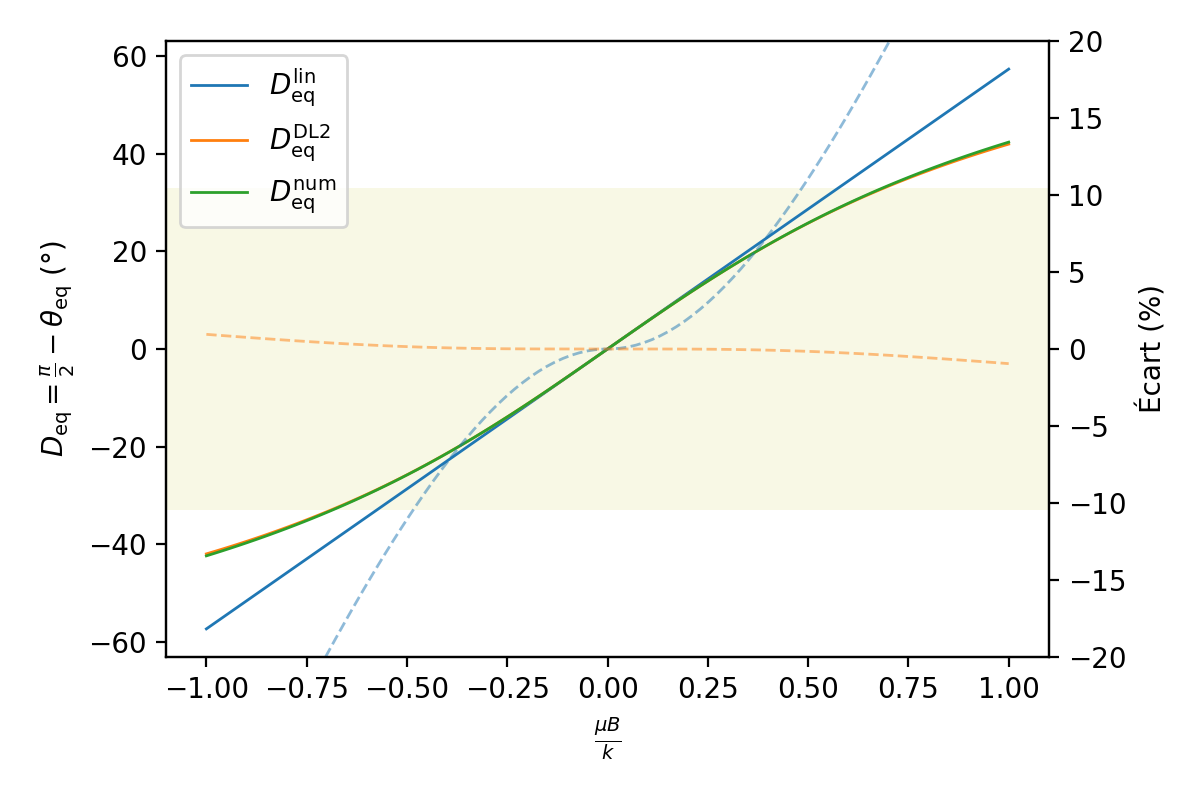
\includegraphics[scale=1]{deviation.png}
    \caption{Déviation de l'aiguille du galvanomètre en fonction du rapport $\tfrac{\mu B}{k}$ proportionnel au courant mesuré.
Les trois courbes pleines représentent les déviations associées aux trois solutions obtenues précédemment dans le cadre de l'approximation linéaire, du développement limité au second ordre et de la résolution numérique.
Les courbes en pointillés montrent l'écart relatif entre les déviations calculées analytiquement (Éq.~\ref{eq:sol_lin} et \ref{eq:sol_dl}) et la résolution numérique (Éq.~\ref{eq:sol_num}).
La plage de déviations matérialisée en jaune pâle représente la gamme de valeurs effectivement mesurables par l'instrument, compte tenu de l'amplitude de mouvement de l'aiguille.}
    \label{fig:deviation}
\end{figure}

\subsubsection{Validité du modèle}

\begin{figure}
    \center
    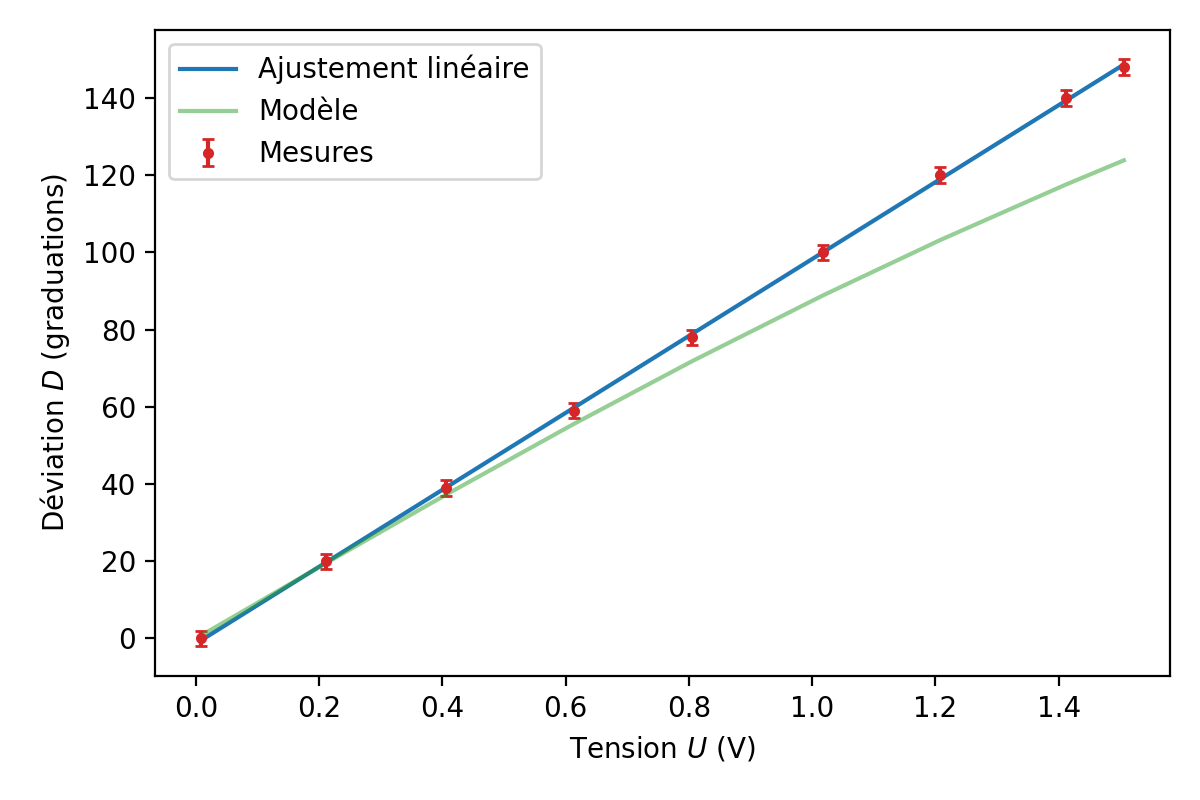
\includegraphics[scale=1]{images/galva_lin.png}
    \caption{Mesure de la déviation en fonction de la tension aux bornes du galvanomètre voltmètre.
    La tension d'une alimentation stabilisée est modifiée et mesurée simultanément à l'aide du galvanomètre et d'un multimètre numérique pour reconstituer la courbe.
    Le calibre du galvanomètre est choisi pour explorer l'ensemble des déviations mesurables.
    De manière surprenante, l'ajustement linéaire semble excellent ($\chi^2_\mathrm{r} \approx \num{0.1}$, $r\approx\num{0.9998}$), y compris aux \og grandes \fg{} valeurs de déviation.
}
    \label{fig:galva_lin}
\end{figure}

\begin{figure}[htbp]
    \center
    \begin{tikzpicture}
        \shade[left color=gray_f!25, right color=gray_f!100] (-4,2) --++ (2,0) --++(0,-4) --++ (-2,0);
        \shade [left color=gray_f!100, right color=gray_f!25] (4,2) --++ (-2,0) --++(0,-4) --++ (2,0);
        \foreach \i in {0,1,...,6} {
            \pgfmathsetmacro\h{-2 +2*\i / 3}
	       \coordinate (A) at (-2,\h);
            \coordinate (B) at (2,\h);
	       \draw[color=red] (A) to[bend left=20*\h] (B);
	       \draw[thick,decorate, decoration={markings,mark=at position 0.5 with{\arrow[red]{stealth}};}] (A) to[bend left=20*\h] (B);
	   }
    \end{tikzpicture}
    \caption{Représentation schématique de quelques lignes de champ au niveau de l'entrefer de l'aimant permanent.}
    \label{fig:entrefer}
\end{figure}

Des mesures rapides effectuées sur les différents appareils n'ont cependant pas montré d'écarts significatifs pour les déviations les plus élevées (Fig~\ref{fig:galva_lin}).
\footnote{La linéarité des graduations sur les cadrants des instruments a été vérifiée à l'aide d'un réglet.}
On peut revenir sur les différentes hypothèses utilisées pour établir le modèle précédent :
\begin{itemize}
\item uniformité du champ $B$ : cette approximation reste valable tant que l'on reste à proximité de l'axe de l'entrefer de l'aimant permanent (Fig.~\ref{fig:entrefer}).
Cependant, puisque la taille du cadre mobile est comparable à celle de l'entrefer, pour des déviations importantes, la bobine explore des régions sensiblement éloignées de l'axe de l'entrefer.
À mesure que l'on s'éloigne de cet axe, le champ magnétique diminue.
Quand l'intensité $I$ est faible, la bobine est proche de l'axe ($\theta\approx\num{\pi/2}$) et elle s'en éloigne quand l'intensité augmente : le couple magnétique devrait donc également diminuer à mesure que la déviation augmente.
Cet effet, qui s'ajoute à la diminution du couple à mesure que le dipôle s'aligne avec le champ, devrait en réalité augmenter la non linéarité de l'affichage : il doit donc être négligeable et l'hypothèse d'un champ magnétique uniforme semble raisonnable ;

\item poids négligeable : dans le cas où l'on devrait considérer le poids de l'aiguille, il faudrait rajouter à l'équation~\ref{eq:mvt} un terme en $\cos\theta$ correspondant au couple du poids, dont la valeur est par ailleurs difficile à estimer sans démonter complètement l'appareil.
On obtient alors l'équation 
\begin{equation}
J\ddot{\theta} = -\mu B \sin \theta - k\left(\theta-\frac{\pi}{2}\right) - \alpha\dot{\theta} - \beta \cos\theta,
\label{eq:mvt_poids}
\end{equation}
où $\beta$ est lié au poids de l'aiguille.
A priori ce terme pourrait convenir : au contraire du moment magnétique, sa valeur augmente avec la déviation et pourrait ainsi compenser la diminution du moment magnétique.
La résolution numérique de l'équation \ref{eq:mvt_poids} dans le régime statique pour plusieurs valeurs de $\beta$ ne laisse cependant pas apparaitre d'amélioration significative.
De plus, les galvanomètres affichent des valeurs identiques, qu'ils soient disposés verticalement ou horizontalement, en accord avec les annonces du fabriquant : \og \emph{Ces galvanomètres fonctionnent dans toutes les positions et sous n'importe quelle orientation} \fg{} (Ann.~\ref{ann:catalogue}). 
\footnote{Le support des galvanomètres les destine à être orientés verticalement (aiguille vers le haut), ce qui a conduit à l'hypothèse selon laquelle le poids de l'aiguille joue un rôle dans la mesure.}
L'approximation réalisée en négligeant le poids semble donc également raisonnable ;

\item force de rappel du ressort spirale : une dépendance plus complexe qu'une simple proportionnalité n'est pas impossible mais il semble que ce type de ressort soit un des rares qui ait un \og comportement vraiment linéaire \fg{} \cite{wiki_ressort} ;

\item géométrie de la bobine : le cadre mobile a une géométrie plus complexe que celle envisagée dans le modèle.
Les détails sont toutefois difficiles à prendre en compte sans rentrer dans une démarche qui dépasse le cadre de ce travail.
Il est par ailleurs difficile d'imaginer que ces détails améliorent la linéarité de l'affichage.
\end{itemize}

\subsubsection{Amélioration du modèle}

Dans ce qui précède, la forme de l'entrefer est très simple (Fig.~\ref{fig:entrefer}).
Toutefois, il est possible de considérer une forme plus évoluée, adaptée à un cadre mobile pivotant (Fig.~\ref{fig:entrefer_cyl}).
\footnote{Sur les instruments utilisés, la forme précise de l'entrefer est difficile à apercevoir sans démonter davantage l'appareil.
Toutefois, elle n'est clairement pas rectangulaire (Fig.~\ref{fig:entrefer}).}
On suppose toujours que le champ magnétique dans l'entrefer est orienté uniquement selon $\ex$ (la convention pour l'orientation des axes reste la même qu'avant).
\footnote{Cette approximation est discutable mais reste raisonnable tant que l'on reste assez proche de l'axe de l'entrefer.}
Le champ magnétique n'est cependant plus uniforme car l'épaisseur $e(\nu)$ de l'entrefer change et dépend de la distance par rapport à l'axe : on peut le noter $B(\nu)\ex$.
Pour calculer le champ magnétique $B(\nu)$, on procède par analogie avec le calcul du champ dans l'entrefer d'un électroaimant \cite{Faroux1998}.
Il apparait que le champ $B$ est inversement proportionnel à l'épaisseur $e(\nu)=2r\cos\nu$ : ici on a donc
\begin{equation}
B(\nu) \propto \frac{1}{\cos\nu}.
\end{equation}

\begin{figure}
\center
\begin{tikzpicture}
\newcommand{\radius}{2}
\newcommand{\angopen}{60}
\coordinate (O) at (0:0);
\pgfmathsetmacro\h{\radius*sin(\angopen)}
\draw[dashed] (O) circle (\radius);
\shade[left color=gray_f!25, right color=gray_f!100]  (-2*\radius, \h) -- (180-\angopen:\radius) arc (-\angopen:\angopen:-\radius) -- (-2*\radius, -\h);
\shade[left color=gray_f!100, right color=gray_f!25] (2*\radius, \h) -- (\angopen:\radius) arc (\angopen:-\angopen:\radius) -- (2*\radius, -\h);
\draw (O) node {$\bullet$} node [below left] {$O$} -- (20:\radius) node [midway, above left]{$r$};
\draw[thick,->,>=stealth] (O)+(1,0) arc (0:20:1);
\draw (O)+(10:1) node[right]{$\nu$};
\draw[dashed] (-2.5*\radius, 0) -- (2.5*\radius, 0);

\coordinate (O) at (8,0,0);
\pgfmathsetmacro\x{.9*\radius*cos(20)}
\pgfmathsetmacro\y{.9*\radius*sin(20)}

\draw[thick] (O) ++ (0,0,-2) --++ (0,0,1);
\draw[thick] (O) ++ (0,0,1) --++ (0,0,1);
\draw[thick, red] (O) ++ (\x, \y,-\radius/2) --++ (0,0,\radius);
\draw[thick] (O) ++ (\x,\y,\radius/2) --++ (-2*\x, -2*\y,0);
\draw[thick, blue] (O) ++ (-\x,-\y,\radius/2) --++ (0,0, -\radius);
\draw[thick] (O) ++ (-\x,-\y,-\radius/2) --++ (2*\x, 2*\y,0);
\draw[thick, decorate, decoration={markings,mark=at position 0.5 with{\arrow[red]{stealth}};}] (O) ++ (\x, \y,\radius/2) --++ (0,0,-\radius);
\draw[thick, decorate, decoration={markings,mark=at position 0.5 with{\arrow[blue]{stealth}};}] (O) ++ (-\x, -\y,-\radius/2) --++ (0,0,\radius);
\end{tikzpicture}
\caption{Un entrefer plus travaillé pourrait expliquer la linéarité du galvanomètre.}
\label{fig:entrefer_cyl}
\end{figure}

La couple des forces de Laplace se calcule en considérant cette fois le cadre mobile comme une bobine formée de $N$ spires carrées de côté $l$, dont l'inclinaison est repérée par l'angle $\nu$. 
\footnote{Cette géométrie est par ailleurs plus proche de la forme réelle du cadre mobile des instruments utilisés.}
La résultante des forces de Laplace qui s'exercent sur un fil de la branche rouge parcouru par un courant $I$ (Fig.~\ref{fig:entrefer_cyl}) s'écrit $-IlB(\nu)\ey$ dont le moment est $-\frac{Il^2B(\nu)}{2}\cos(\nu)\ez$.
Le couple exercé sur le cadre mobile est donc
\footnote{Cette fois, on obtient un terme en cosinus mais cela est simplement dû à la définition de l'angle utilisé pour repérer l'inclinaison du cadre mobile : en effet, $\theta = \nu + \pi/2$.}
\begin{equation}
\vec{\Gamma}_B = -NIl^2B(\nu)\cos(\nu)\ez.
\end{equation}
En utilisant le résultat précédent concernant la dépendance du champ $B$ avec l'angle $\nu$, on obtient finalement
\begin{equation}
\vec{\Gamma}_B \propto NIl^2 \ez,
\end{equation}
où le facteur de proportionnalité dépend simplement de l'aimantation de l'aimant permanent.

Cette équation est remarquable puisque cette fois, le moment magnétique ne dépend pas de l'inclinaison du cadre !
L'équation du mouvement (Éq.~\ref{eq:mvt}) devient linéaire, sa résolution analytique en régime permanent est alors possible et conduira à une déviation proportionnelle à l'intensité qui parcours le galvanomètre.
Avec ce dernier modèle, on explique très bien les résultats obtenus expérimentalement (Fig.\ref{fig:galva_lin}).

\subsection{Remarques sur la conception des appareils}

La présence de frottements lors des mouvement du cadre mobile est essentielle au bon fonctionnement de l'appareil : ils permettent de s'assurer que l'aiguille atteigne sa position d'équilibre \og sans oscillation et néanmoins avec exactitude \fg{} (Ann.~\ref{ann:catalogue}).
Les appareils étudiés sont \emph{apériodiques}, ce qui semble faire référence à cette absence d'oscillation lors du régime transitoire : on pourrait contraindre la valeur de $\alpha$ dans notre modèle avec cette contrainte.

La longévité de la calibration des instruments repose notamment sur la constance du champ magnétique produit par l'aimant permanent.
Dans le catalogue constructeur (Ann.~\ref{ann:catalogue}), on peut également lire que le principe de fonctionnement de ces instruments \og \emph{permet de réaliser des appareils de mesure dont la permanence de l'étalonnage peut-être considérée comme pratiquement absolu} \fg{}.
Derrière cet argument de vente percutant se cachent deux vérités :
\begin{itemize}
\item \og la très faible force magnétomotrice développée par le courant traversant les spires du cadre mobile et qui est sans action appréciable sur l'aimant permanent \fg{} ;
\item la forme torique de l'aimant conduit naturellement à des lignes de champs quasiment fermées, ce qui préserve l'aimantation de l'aimant.
\end{itemize}


\section{L'ampèremètre}

\begin{figure}[htbp]
    \center
    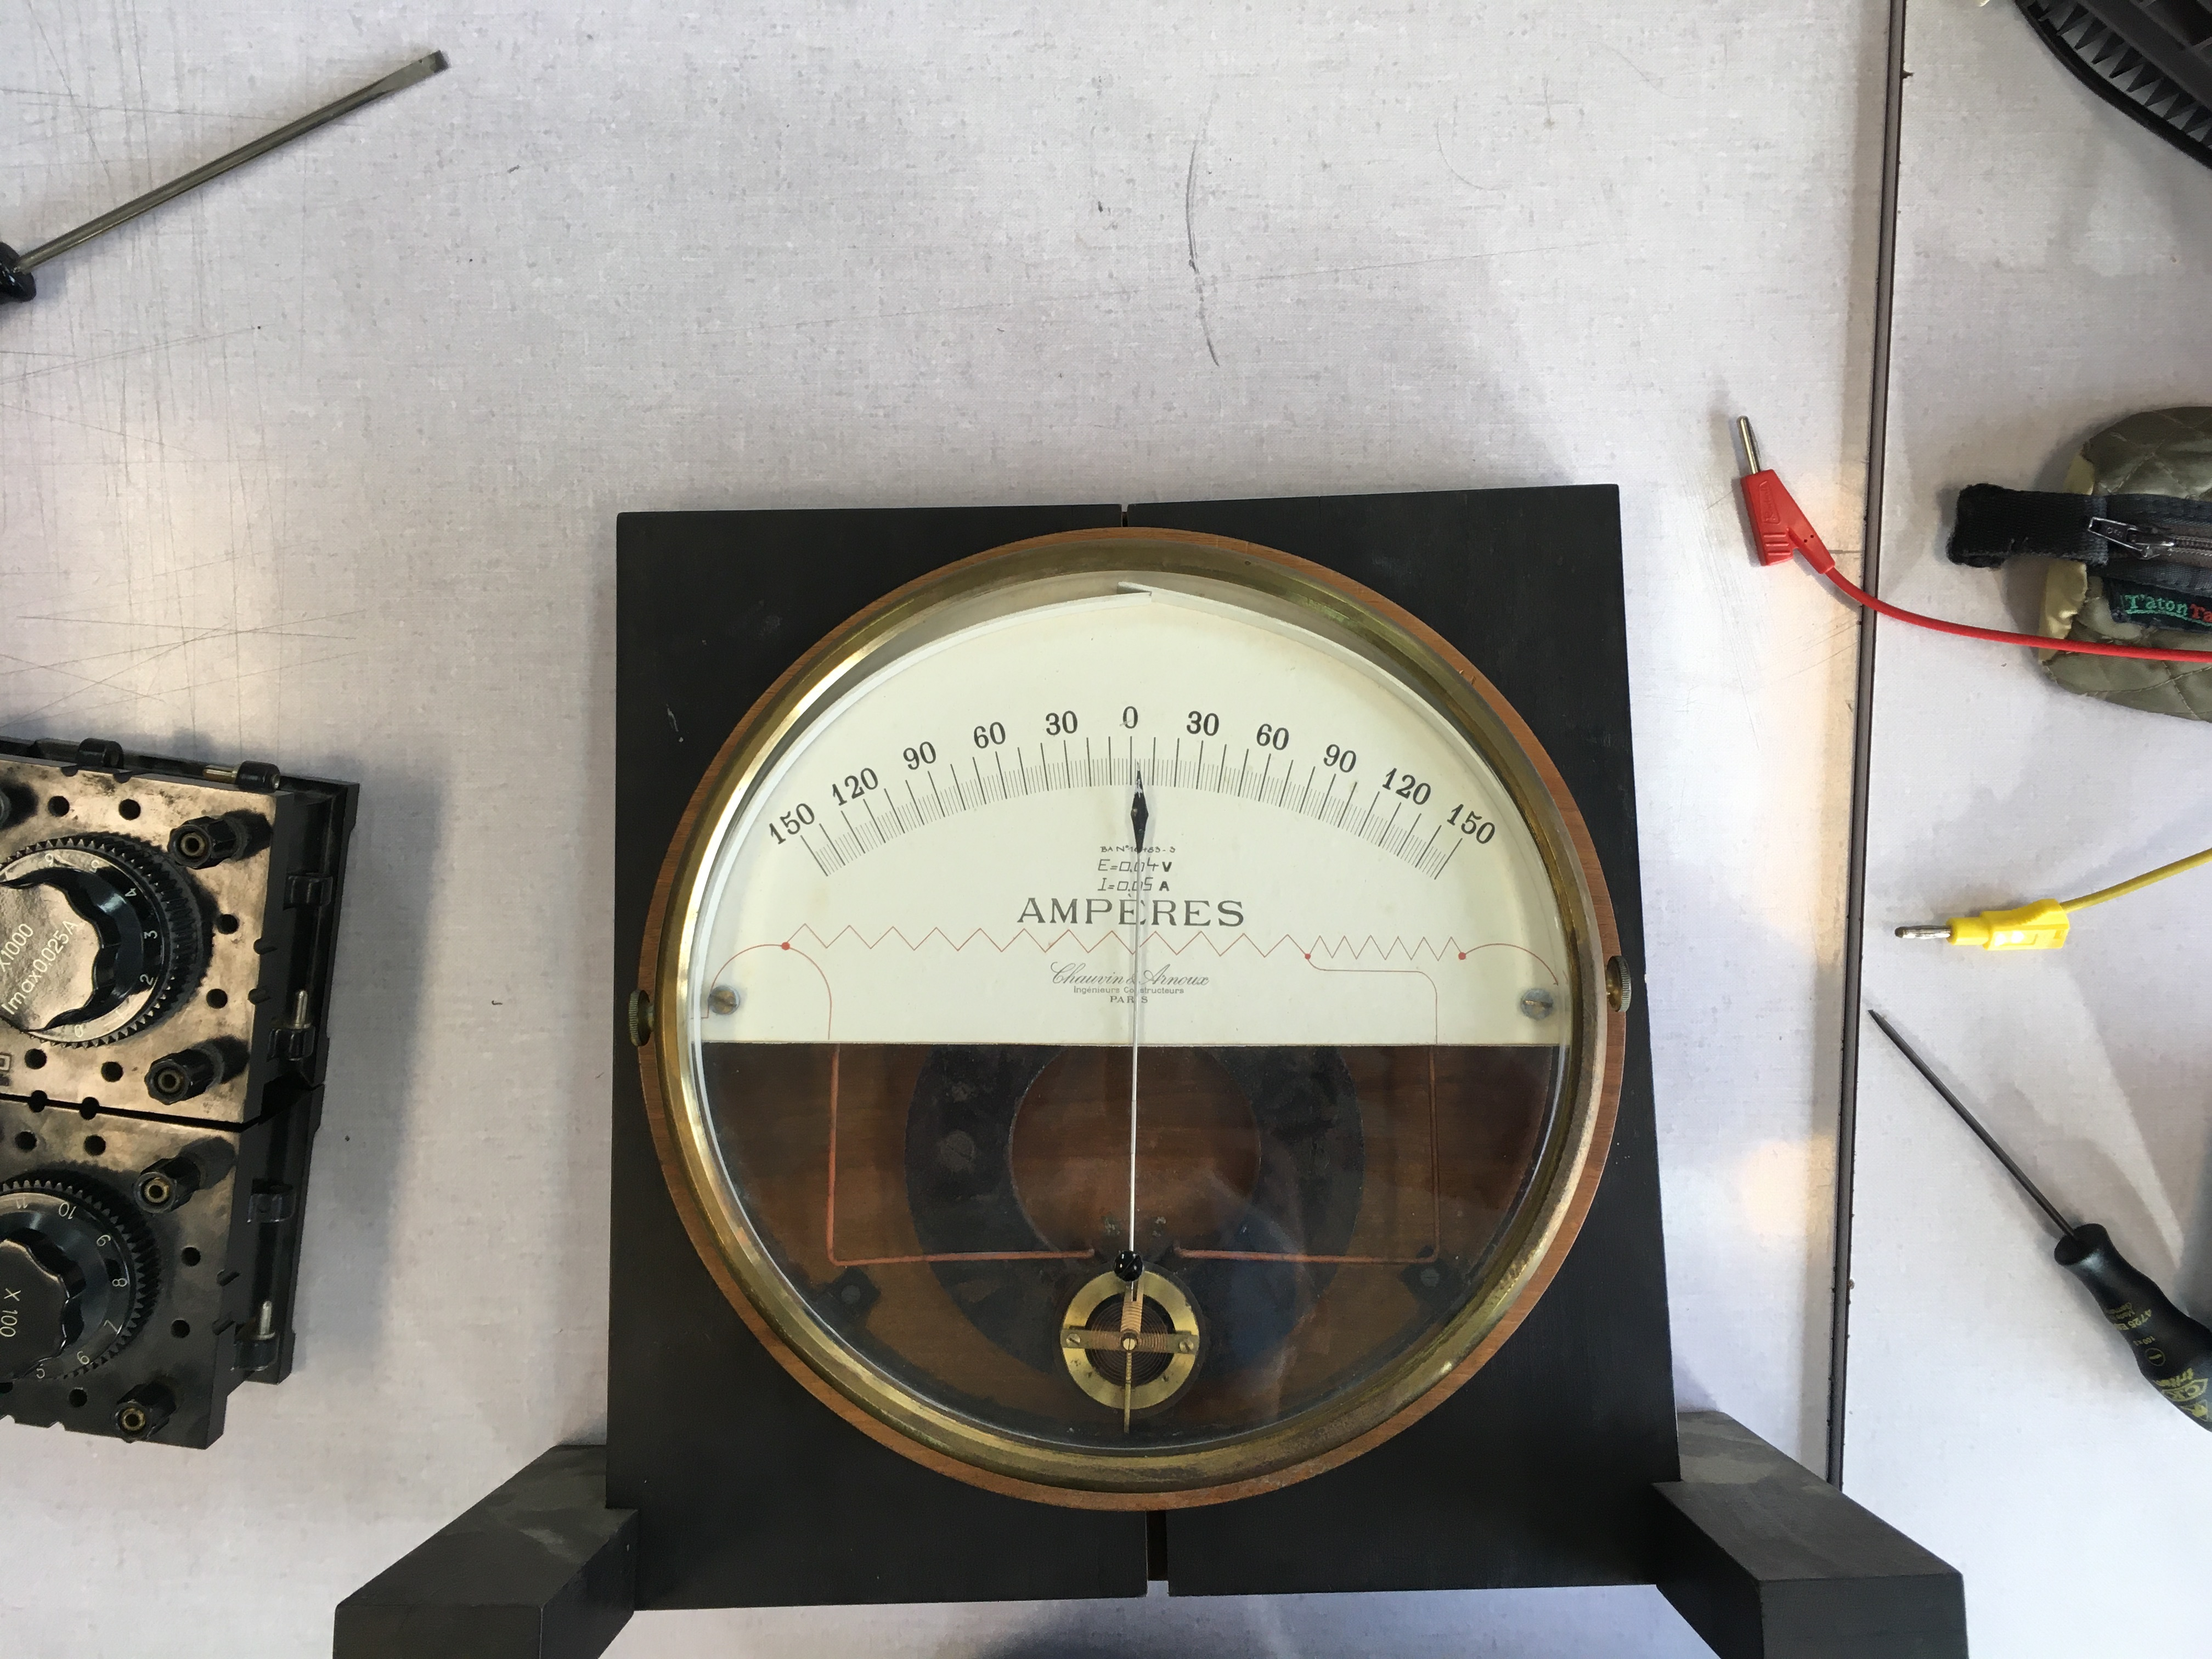
\includegraphics[height=300 pt, trim=800 0 700 800, clip]{images/IMG_4012.JPG}
    \caption{Le galvanomètre ampèremètre avant toute manipulation.}
    \label{fig:galva_amp_av}
\end{figure}

L'ampèremètre auquel on s'intéresse ici était commercialisé par Chauvin \& Arnoux, probablement au cours de la première moitié du XX\textsuperscript{ème} siècle.
Il s'agit d'un modèle de \SI{25}{cm} de diamètre, qui peut fonctionner quelque soit le sens du courant (continu) et dont le cadrant possède 150 graduations dans chaque sens.
Bien que ce modèle précis ne soit pas dans le catalogue du fabricant présenté en annexe (Ann.~\ref{ann:catalogue}), on en trouve un modèle très similaire, qui était vendu au prix de 130 francs en 1915, soit environ 360 euros actuels \cite{Alexandre2014}.
Le galvanomètre est monté sur un support en bois qui le maintien à la verticale.

Quand on le récupère sur son étagère pour l'examiner, le galvanomètre est en bon état et à peine poussiéreux.
Comme premier test, on mesure sa résistance interne à l'aide d'un multimètre numérique : la résistance lue est de l'ordre de \SI{1}{\ohm}, trop faible pour être mesurée précisément avec cet appareil.
De plus lorsque le multimètre est connecté aux bornes du galvanomètre, l'aiguille de ce dernier bouge de quelques graduations : il semble donc en état de marche.
Il y a toutefois quelques problèmes mineurs :
\begin{itemize}
    \item en l'absence de courant, l'aiguille n'est pas centrée en zéro, et le réglage de l'\og offset \fg{} est en bout de course ;
    \item le système de graduation est mystérieux ;
    \item l'aiguille et notamment sa pointe sont légèrement tordues.
\end{itemize}
Une expérience rapide permet de s'assurer qu'il permet de réaliser des mesures (Fig.~\ref{fig:galva_amp_mes}).

\begin{figure}[htbp]
    \center
    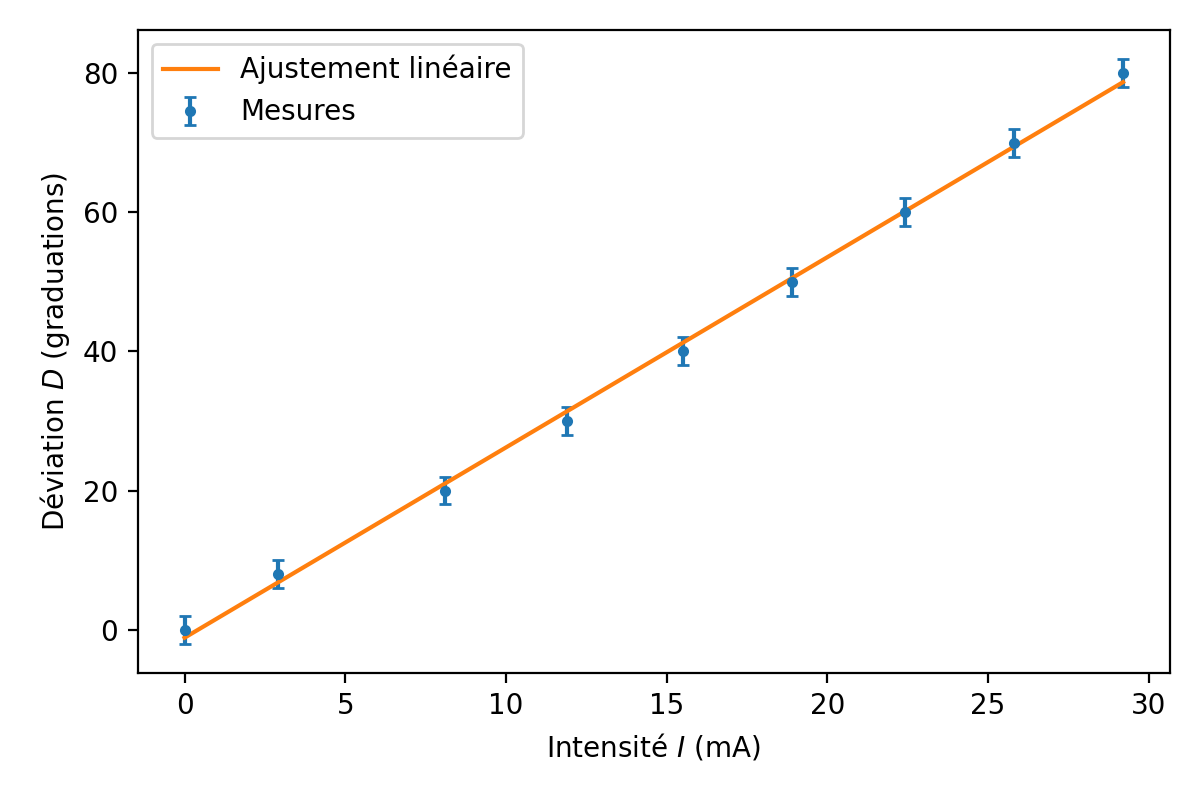
\includegraphics[scale=1]{images/mesure.png}
    \caption{Vérification du fonctionnement de l'instrument du galvanomètre ampèremètre.
    Le circuit utilisé est une simple résistance de \SI{1}{\kilo\ohm} branchée à la sortie d'une alimentation variable stabilisée en tension.
    Le galvanomètre et un multimètre numérique utilisé comme ampèremètre sont branchés en série avec la résistance.
    On fait varier la tension de l'alimentation pour obtenir la courbe ci-dessus.
    Les barres verticales correspondent aux incertitudes de mesure avec le galvanomètre, correspondant à une graduation.}
    \label{fig:galva_amp_mes}
\end{figure}

En supposant que le galvanomètre fonctionne toujours comme en sortie d'usine, cette série de mesure permet de comprendre l'échelle de graduation.
Le coefficient directeur de la droite obtenu lors de l'ajustement des mesures donne \SI{2.74(7)}{graduation\per\milli\ampere}.
On compare aux valeurs indiqués sur le cadrant : comme le suggère la notice, si la graduation la plus élevée (150) correspond au courant maximal mesurable avec l'instrument ($I_\mathrm{max}=\SI{0.05}{\ampere}$), le coefficient directeur devrait être de \SI{3}{graduation\per\milli\ampere}.
Ces deux valeurs sont raisonnablement proches à ce stade pour supposer que la dernière graduation correspond à la valeur maximale indiquée sur le cadrant.
\footnote{La graduation du cadrant en 150 divisions semble être commune à de nombreux modèles commercialisés par Chauvin \& Arnoux, même s'ils proposent d'autres échelles : 100, 125 et 150 divisions.}

Pour en apprendre davantage sur l'instrument, nous décidons de le démonter :
\begin{itemize}
    \item on l'enlève de son support vertical en bois en dévissant les quatre vis qui l'y maintiennent ;
    \item on retire la vitre de protection, maintenu par une bague en laiton ajustée au cylindre qui fait le tour de l'instrument.
    Pour cela, on procède avec précaution, en exerçant à l'aide d'un gros tournevis un effort sur le dessous de la bague pour la soulever, en prenant appui sur les bornes de branchement de l'instrument pour faire un levier.
    La vitre repose simplement sur deux grands anneaux, l'un métallique et l'autre cartonné ;
    \item on retire le cadrant en dévissant les deux vis en laiton, puis en le faisant pivoter à droite, tout en maintenant l'aiguille complètement à gauche.
\end{itemize}
On se retrouve alors l'intérieur de l'instrument mieux visible (Fig.~\ref{fig:galva_amp_int}).

En plus des fils qui alimentent le cadre mobile, on remarque la présence d'un fil en forme de ressort qui relie les bornes du galvanomètre.
Dans la notice (Ann.~\ref{ann:catalogue}), il est indiqué que la bobine du cadre mobile est de l'ordre de \SI{0.5}{\ohm}.
Il est par ailleurs indiqué qu'\og une résistance en métal à coefficient de température nul est ajoutée pour le tarage de l'appareil \fg{}.
Il semblerait que ce soit cette résistance qui fixe le calibre de l'appareil : plus la résistance est faible, plus on pourra mesurer des courants intenses puisque la plupart du courant passera à travers cette résistance.
On parle de \emph{shunt}.
Les indications du cadrant ($I_\mathrm{max}=\SI{0.05}{A}$ et $U_\mathrm{max}=\SI{0.04}{V}$) permettent de déduire la résistance équivalente de l'ensemble, correspondant à la résistance interne de l'appareil : on trouve \SI{0.8}{\ohm}.
Cette résistance est difficilement vérifiable en raison de sa faible valeur.



Problème : réglage du zéro impossible, légèrement poussiéreux, fonctionne, pointe légèrement tordue

Problème survenu plus tard : brasure défaillante et grille pain sur le fil ressort alors que la bobine n'était pas raccordée.

\begin{figure}[htbp]
    \center
    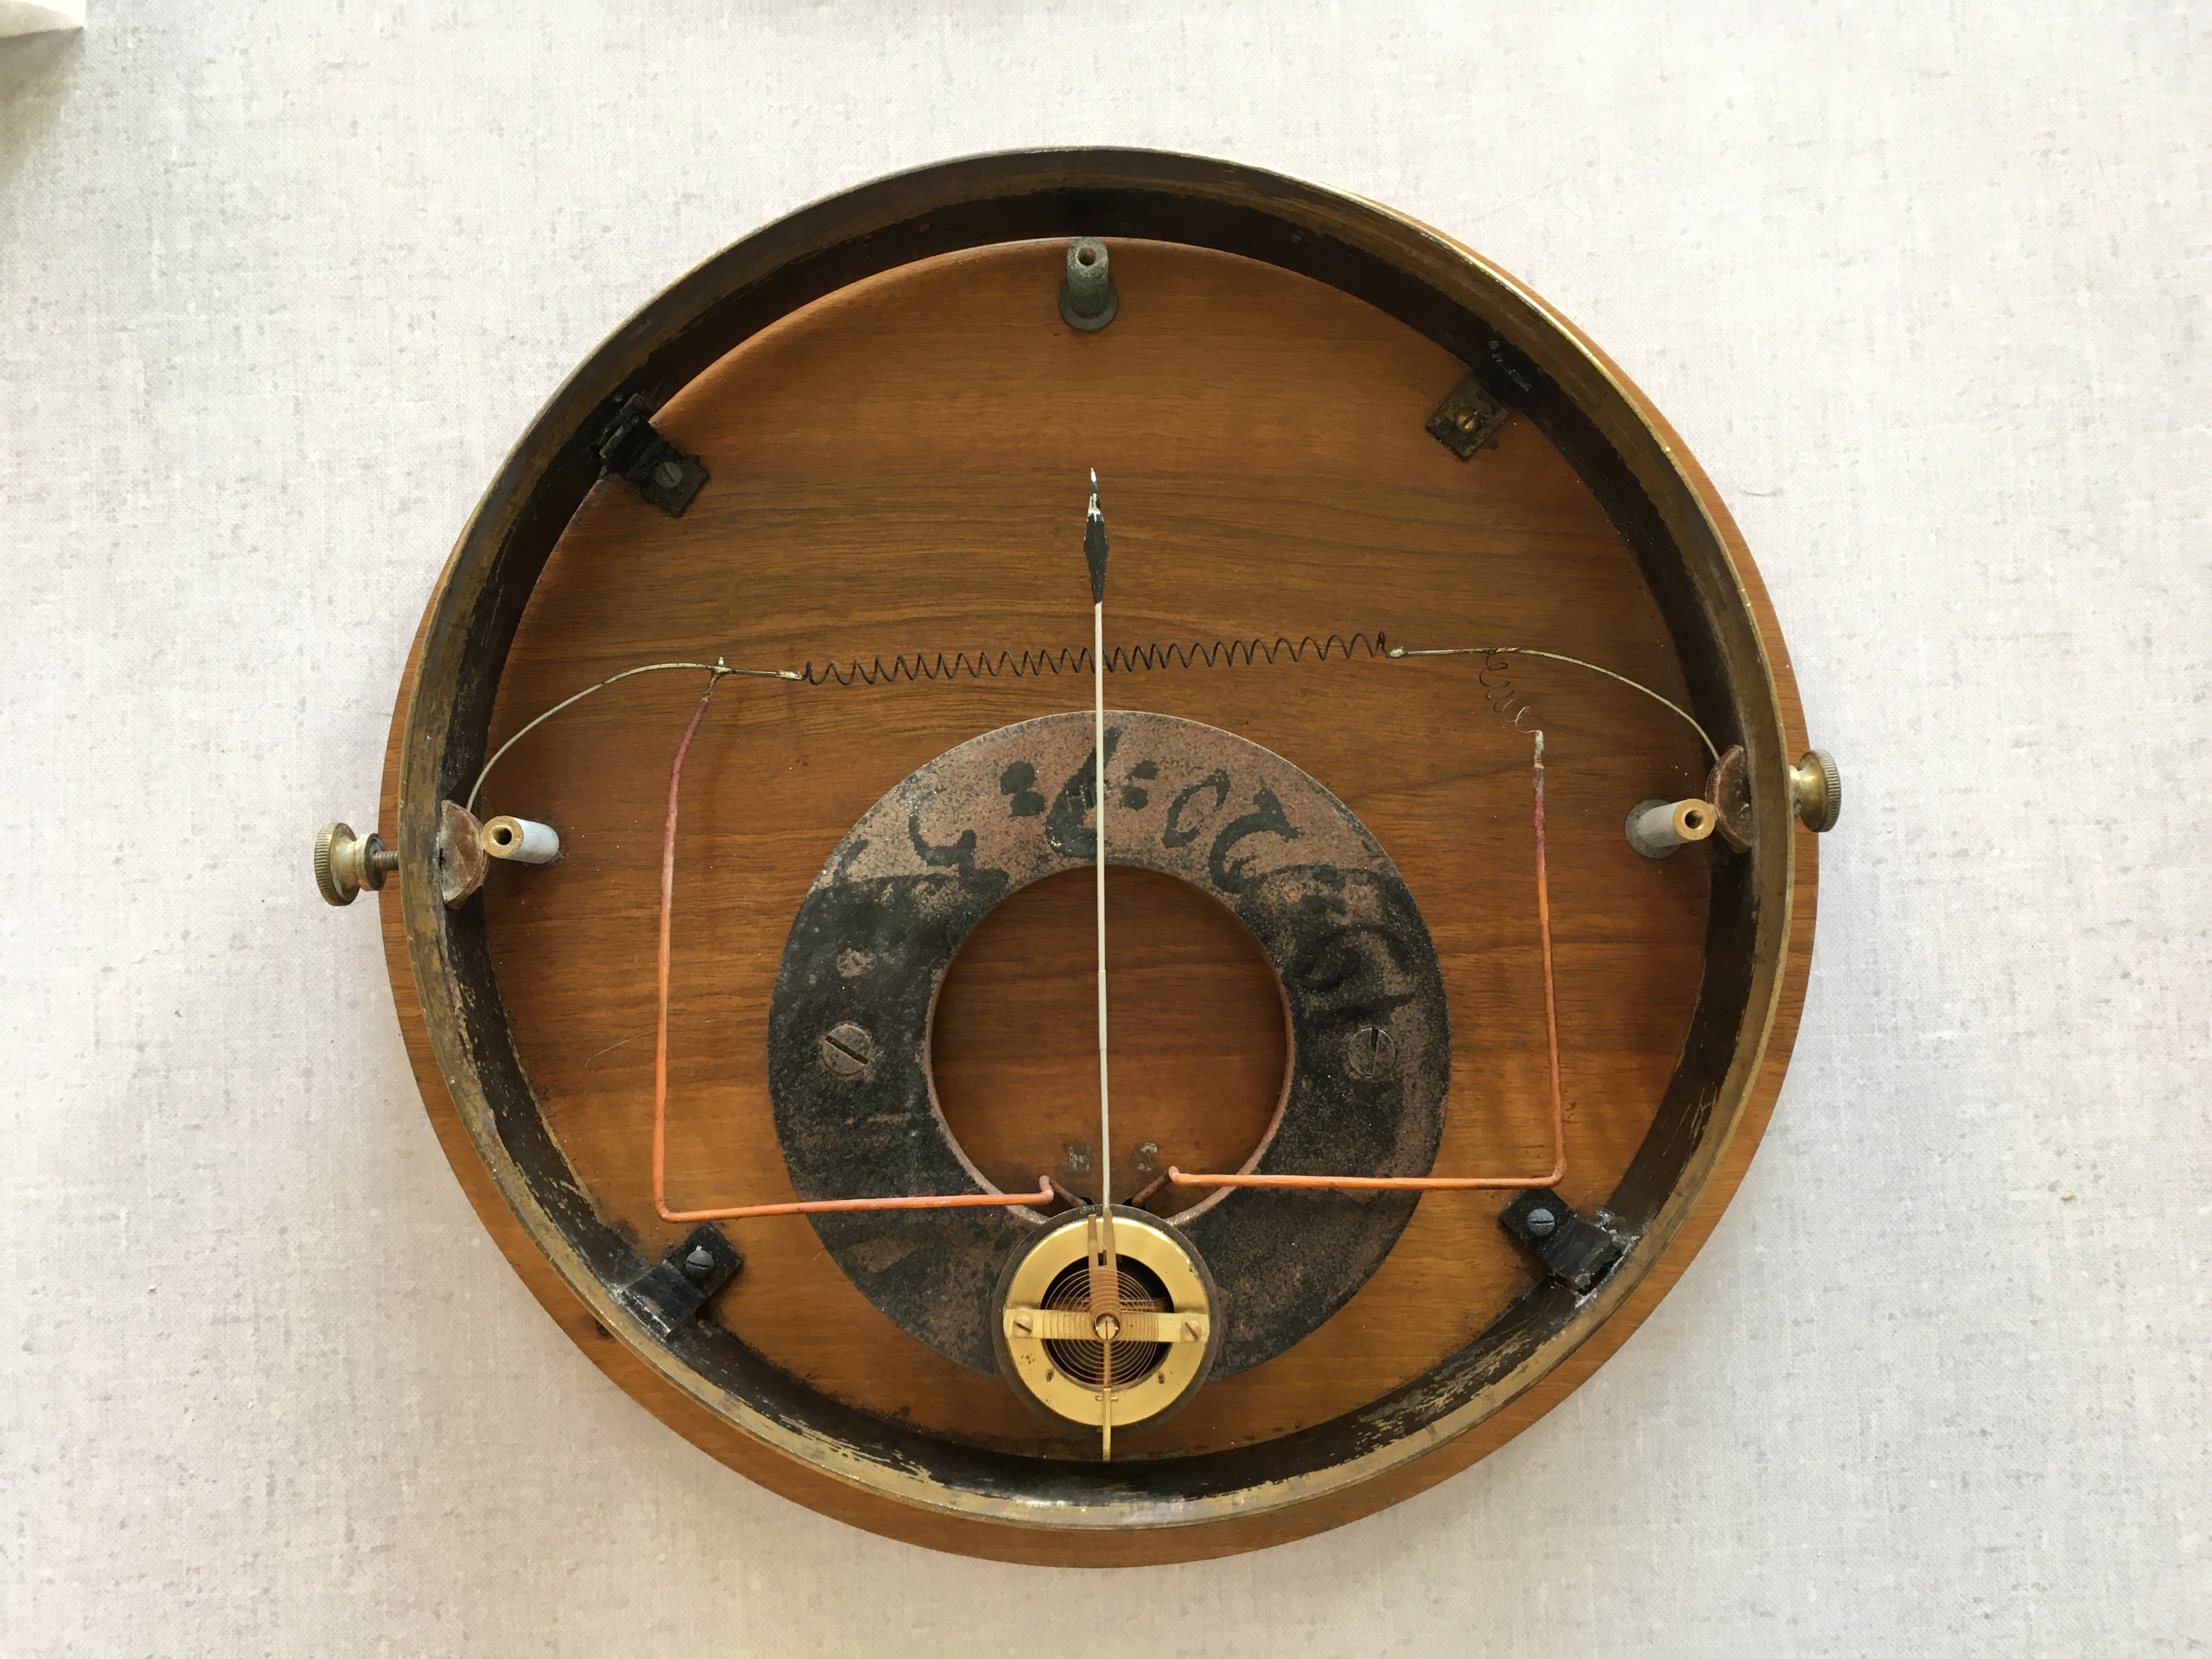
\includegraphics[height=300 pt, trim=500 100 600 200, clip]{images/IMG_4037.JPG}
    \caption{Le même galvanomètre, une fois la vitre et le cadrant retirés.}
    \label{fig:galva_amp_int}
\end{figure}



\section{Le voltmètre}



\section{Expérience type}



\section*{Conclusion}
\addcontentsline{toc}{section}{Conclusion}

\newpage
\appendix

\bibliography{biblio.bib}
\addcontentsline{toc}{section}{Références}

\newpage
\appendix

\addcontentsline{toc}{section}{Annexes}

\section{Extraits du catalogue Chauvin \& Arnoux (1915)}
\label{ann:catalogue}

Le catalogue complet est disponible en cliquant sur le lien ci-dessous :

\noindent
\href{http://cnum.cnam.fr/CGI/fpage.cgi?M9857.1/1/100/137/104/135}{http://cnum.cnam.fr/CGI/fpage.cgi?M9857.1/1/100/137/104/135}

Les pages qui concernent les instruments étudiés dans ce rapport sont rapportées ci-après.

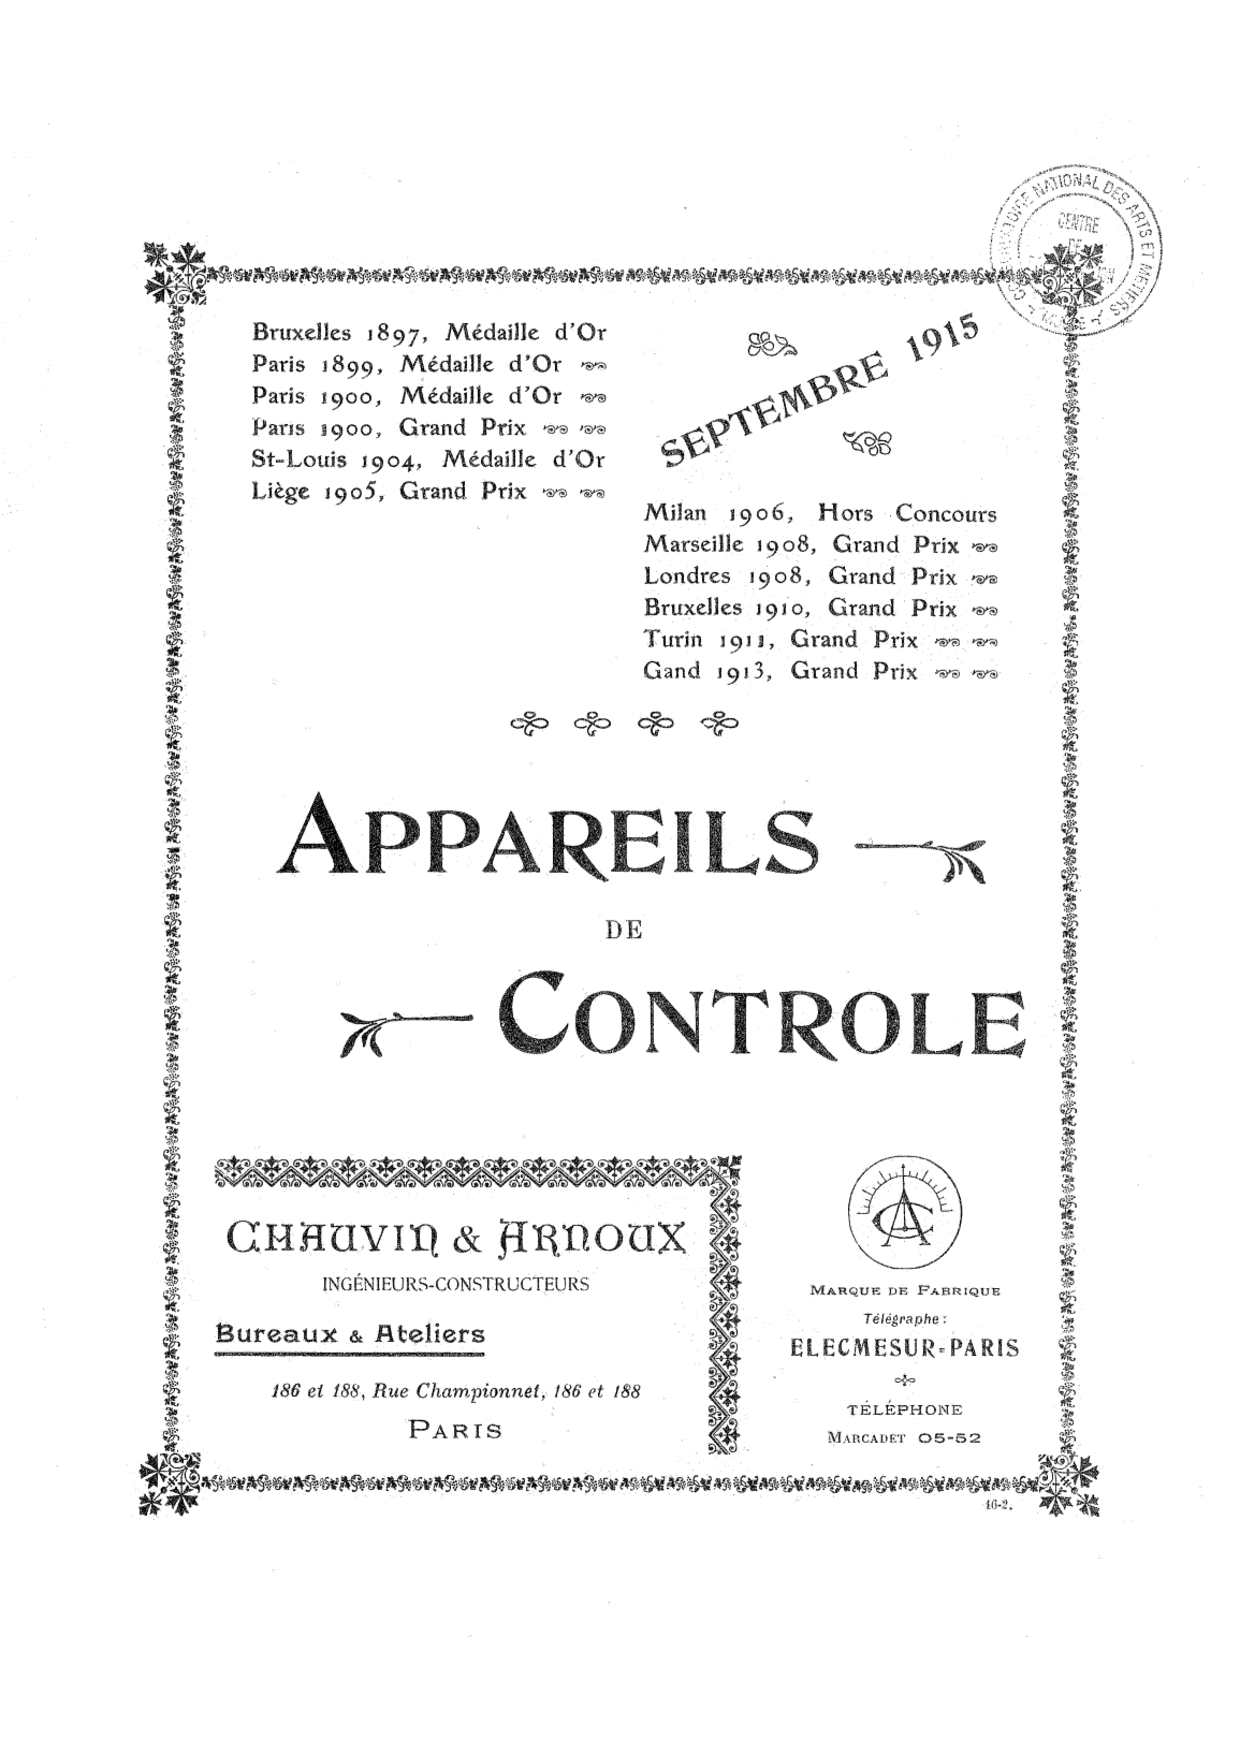
\includepdf[pages=-]{images/chauvin_arnoux.pdf}
\end{document}